\documentclass[a4paper]{article}

%%%% THESE VARIABLES SHOULD BE UPDATED EACH YEAR OF IPC %%%%
\def \compDate {April 23, 2016}
\def \competitionChairName {Aleksander Eskilson}
\def \competitionChairEmail {aeskilson@ku.edu}
%%%%  THESE VARIABLES SHOULD BE UPDATED WHEN NECESSARY  %%%%
\def \DOMJudgeURLShort {http://bit.ly/1jVYOw9}
\def \DOMJudgeURLLong {http://ec2-54-88-68-156.compute-1.amazonaws.com/public/}
\def \previousProblemsRepo {https://github.com/acmatku}
%%%%%%%%%%%%%%%%%%%%%%%%%%%%%%%%%%%%%%%%%%%%%%%%%%%%%%%%%%%%

\usepackage[english]{babel}
\usepackage[margin=1in]{geometry}
\usepackage[utf8]{inputenc}
\usepackage{amsmath}
\usepackage{graphicx}
\usepackage{listings}
\usepackage{color}
\usepackage[parfill]{parskip}
\usepackage[colorinlistoftodos]{todonotes}
\usepackage[colorlinks=true,urlcolor=blue,linkcolor=blue]{hyperref}
\usepackage{fancyhdr}

\pagestyle{fancy}

\definecolor{mygreen}{rgb}{0,0.6,0}
\definecolor{mygray}{rgb}{0.5,0.5,0.5}
\definecolor{mymauve}{rgb}{0.58,0,0.82}

\lstset{
    basicstyle=\ttfamily,
    numbers=left,
    numbersep=8pt,
    showspaces=false,
    showstringspaces=false
    backgroundcolor=\color{white},
  	breaklines=true,
  	captionpos=b,
  	commentstyle=\color{mygreen},
  	escapeinside={\%*}{*)},
  	keywordstyle=\color{blue},
  	stringstyle=\color{mymauve}, 
}

\title{ACM@KU, Intramural Programming Competition: \\ 
Rules, Resources, and Examples}

\date{\compDate}

\author{The Association for Computing Machinery at the University of Kansas}

\begin{document}
\maketitle

\tableofcontents

\newpage

\section{Introduction}

The ACM@KU Intramural Programming Competition is an ACM-style programming competition designed to test your knowledge of programming as a tool for general problem solving. Languages of the competition will include but not be necessarily limited to the following:
\begin{center}
    C \\
    C\texttt{++} \\
    Clojure \\
    Haskell \\
    Java 8 \\ 
    Lua \\
    PHP \\
    Python (v. 2.7 and 3.4) \\
    Ruby \\
\end{center}

\newpage

\section{Contact}

If you have questions regarding the competition, please feel free to contact:
\begin{center}
    \competitionChairName \\
    IPC Chair \\
    \url{\competitionChairEmail} \\
\end{center}

\newpage

\section{Rules}

You will be given a docket describing a total of 10 programming challenges, of varying difficulty, and arranged in mixed order. You will be allotted five hours in a single block of time, to write solution programs for these challenges. An automated system called DOMJudge provides a website interface, \url{\DOMJudgeURLShort} or its full url, \url{\DOMJudgeURLLong}, where you can submit your solutions for judging, receive feedback, and check a running scoreboard and clock. Before the actual day of the competition, a test competition will be available here. The login username: \texttt{test}, password: \texttt{pass}, will allow you to browse the interface and even submit a solution to the problems of the test contest. Here, you can test submitting your programs for automated judging. 

All problems will be described in a uniform fashion: An introduction to the problem will set up the scenario and describe what challenge you must write a program to solve. It will then describe how the input your program must read will be structured, and it will prescribe how the program's output must be formatted in order to be read correctly. An example of input and output will be provided for you to check your program against. 

\textbf{Note}: when your program is actually judged, different input data will be used, but the formatting will be the same as described in the problem. Pay very special attention to the section describing how to properly write your programs to accept input from DOMJudge and how to structure our output.

Each correct problem is worth 1 point, so whichever competitor completes the most problems out of 10 will be designated the winner. In the case of ties, time (as marked in seconds, running from the beginning of the competition) will be used as a tiebreaker. So if more than 1 competitor completes all 10 problems, the first to have done so is the winner. You may submit your solutions for judging as many times as you need to, but you should be aware that each time you submit a solution that is judged to be incorrect, you will receive a time penalty that will add to your total time, so it is best to work hard to ensure your program is correct before submitting for judging. However, even if your submission turns out to be wrong, you should feel free to rework it until you get it right or decide to move on to another problem. 

You must compete by yourself. You will be allowed use of the Internet and any books on your programming language may be used during the competition. You may choose to either use the Linux or Windows machines of the EECS Labs, or you may bring your own laptop. For students who do not have KU EECS accounts and who do not bring their own laptops, guest accounts will be provided. 

\textbf{Note}: DOMJudge runs on an Ubuntu 14.04 LTS distro. All solutions then are compiled against the freely available compiler or interpreter for that distro. If you use special packages beyond your language's standard library or you use modified compilers or interpreters on your own machine, we cannot guarantee it will run precisely the same on the judging machine.

\newpage

\section{DOMJudge}

\subsection{Summary}
Here we include a short summary of the DOMJudge system interface, the webportal by which you will submit your solutions for automated judging. The single constraint of this system is that your programs \textbf{must} be written to accept their input from \texttt{stdin} and write their output to \texttt{stdout} (also sometimes referred to as \textit{writing to the console}). We talk a little more about what this means in the examples portion of this section. What follows is an introduction to the interface.

\subsection{Interface}
A web URL will be provided to you from which you will gain access to the DOMJudge submission interface. From your team page, \url{http://example.com/domjudge/team}, you will select \textbf{Select file...} in the left column and select the file of your source code to submit. By default, the problem is selected from the base of the filename and the language from the your file's file extension. 

Viewing scores, submissions, and sending and reading clarification requests is done through the web team interface, \url{http://example.com/domjudge/team}. 

\begin{figure}[p]
    \centering
    \fbox{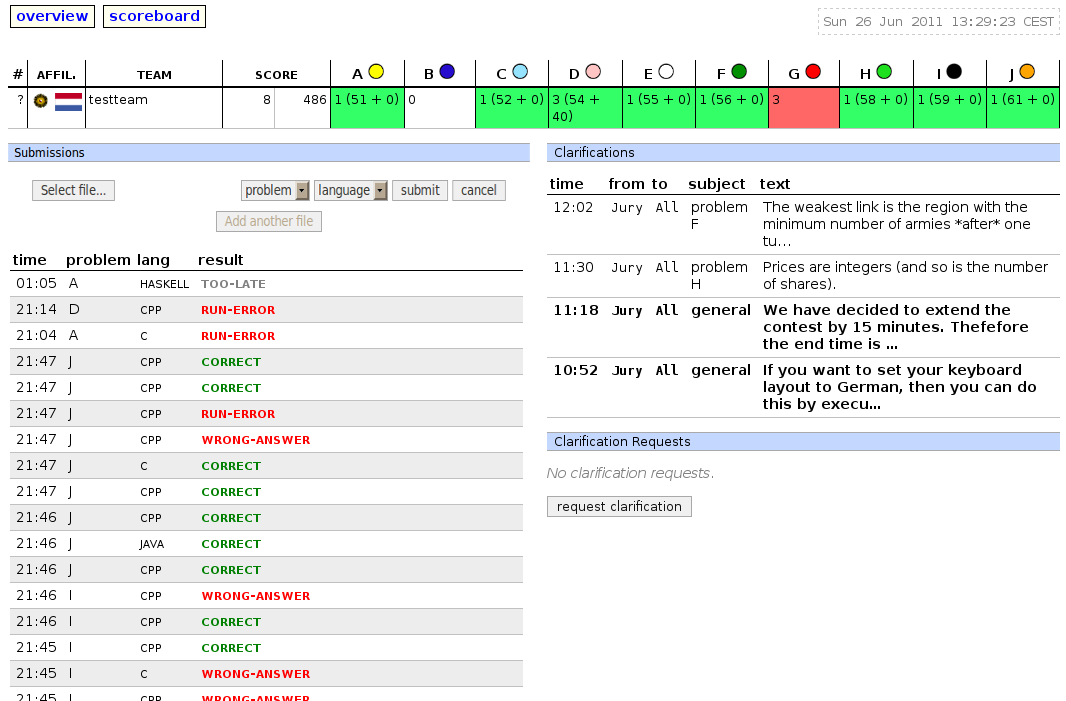
\includegraphics[width=14cm]{assets/team-overview.png}}
    \caption{the web team interface overview page}
    \label{fig:team-overview}
\end{figure}

\begin{figure}[p]
    \centering
    \fbox{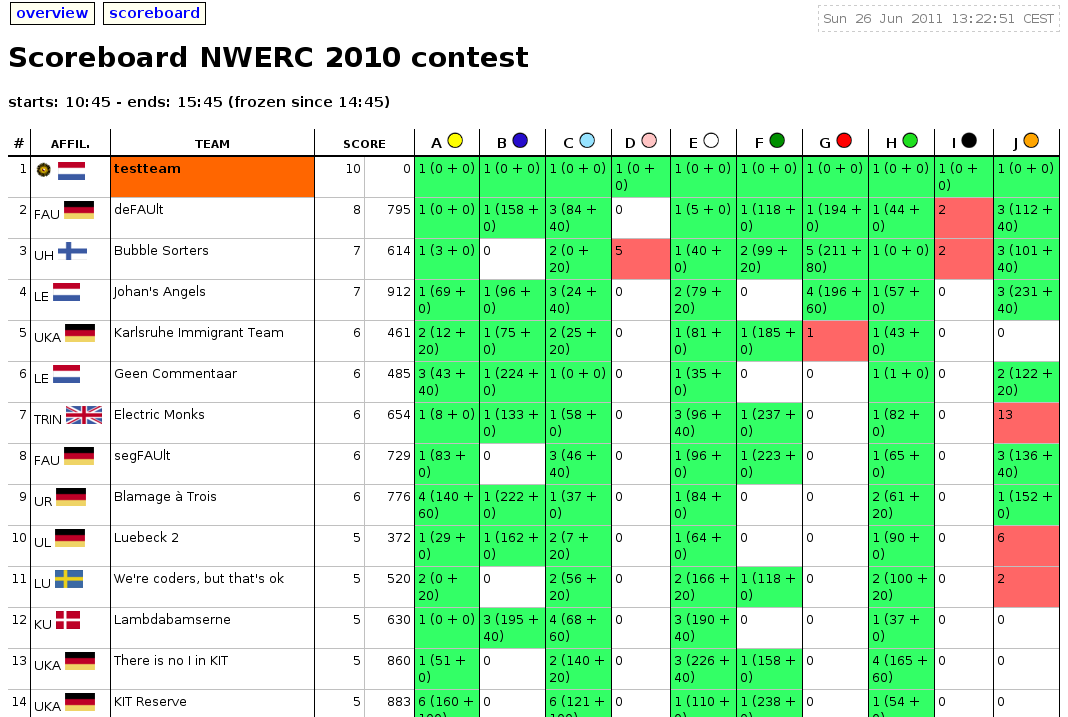
\includegraphics[width=14cm]{assets/team-scoreboard.png}}
    \caption{the scoreboard webpage}
    \label{fig:team-scoreboard}
\end{figure}

The left column of the team interface shows your teams's row in the scoreboard: your position and the which problems you attempted and which you solved. Via th menu, you can view the public scoreboard page with scores of all the teams. The score column lists the number of problems solved and the total penalty time. Each cell in the problem column lists the number of submissions, and if th problem was solved as well as the time of the first correct submission for that problem since the contest start. Submissions can have the following resuts:

\begin{description}
    \item[CORRECT:]
        The submission passed all tests: you solved this problem!

    \item[COMPILER-ERROR:]
        There was an error when compiling your program. On the submission
        details page you can inspect the exact error (this option might be
        disabled).

    \item[TIMELIMIT:]
        Your program took longer than the maximum allowed time for this
        problem. Therefore it has been aborted. This might indicate that your
        program hangs in a loop or that your solution is not efficient
        enough.

    \item[RUN-ERROR:]
        There was an error during the execution of your program. This can have
        a lot of different causes like division by zero, incorrectly
        addressing memory (e.g. by indexing arrays out of bounds), trying to
        use more memory than the limit, etc.
        Also check that your program exits with exit code 0!

    \item[NO-OUTPUT:]
        Your program did not generate any output. Check that you write to
        standard out.

    \item[WRONG-ANSWER:]
        The output of your program was incorrect. This can happen simply
        because your solution is not correct, but remember that your output
        must comply exactly with the specifications of the jury.

    \item[PRESENTATION-ERROR:]
        The output of your program has differences in presentation with the
        correct results (for example in the amount of whitespace). This will,
        like WRONG-ANSWER, count as an incorrect submission. This result is
        optional and might be disabled.

    \item[TOO-LATE:]
        Bummer, you submitted after the contest ended! Your submission is
        stored but will not be processed anymore.
\end{description}

You are allowed to communicate with the jury, we omniscient few who oversee the entirety of the competition namelessly, and behind the inscrutability of teletype terminals, through the use of clarifications. These can be found in the right column of your team page. Both clarification replies from the jury and requests sent by your are displayed there. 

There is also a button to submit a new clarification request to the jurry. This request is only readable for the jury and they will respond as soon as possible. If the jury deems an answer relevant to everyone, it will be viewable to everyone. 

\subsection{Testing}
The DOMJudge system is fully automated. Once input/output files have been prepared to verify your program, no other human element is necessary in scoring besides clarifications on the part of the jury. But this is how it works:

With the web interface you can submit the source code of your solution to the jury. Note that you must send your source code, not a compiled version of the program. Your solution is then sent over the network to a judging computer that will automatically compile or interpret your solution and pipe the proper input file to the program. The output of your program will then be compared against the validated output file. If your output matches the expected output, your program is correct. If not, you will receive some information about what went wrong before you go back to the drawing board.

\textbf{Note}: because DOMJudge provides testing inputs as files from \texttt{stdin}, you should not write your programs to expect input from a human source, such as through the keyboard.

On your local machine, you could test each of your solutions either in a Bash terminal environment, or by using the \texttt{stdin} environment variable of your preferred IDE. To test your solutions against sample inputs, copy the input to a text file like \texttt{input.txt}. Then invoke your interpreter on your solution or run your compiled executable, and use the caret operator, \texttt{<}, to pipe the file into the program's \texttt{stdin}. A terminal command like one of the following should work:

\texttt{python my-solution.py < input.txt}

\texttt{./my-c-executable < input.txt}

Your program should then print the results to the terminal for you, that is, to \texttt{stdout}.

\section{Input/Output Examples}
Here we define how you must write your program to read from \texttt{stdin} and write to \texttt{stdout} for the languages supported by this competition. We do this through annotation of two example programs. The purpose of this section is to expose you to the common input/output functions of your language that will allow your program to accep intput from DOMJudge and write output back to it.
\newpage

\subsection{Hello World}
\textbf{Description:} Write a program to send a friendly greeting! 

\textbf{Input:} Write a program to read a list of names headed by an integer from \texttt{stdin}. The first line will be an integer representing the number of lines to read. Each subsequent line will be a single name.

\textbf{Output:} On a new line for each, print out to \texttt{stdout} the name you read as part of the string ``Hello \textless name\textgreater!''.

\textbf{Sample:}

\begin{tabular}{|p{0.47\textwidth}|p{0.47\textwidth}|}
    \hline
    \textbf{input} & \textbf{outout} \\
    \hline
    \begin{verbatim}
    3
    World
    Alan
    Ada
    \end{verbatim} &
    \begin{verbatim}
    Hello world!
    Hello Alan!
    Hello Ada!
    \end{verbatim} \\
    \hline
\end{tabular}
\newpage

A solution for the problem in C:
\lstinputlisting[language=C]{examples/01/say-hello.c}

Here, we note that C uses the \texttt{scanf} function to read from \texttt{stdin} and \texttt{printf} to write to \texttt{stdout}. It declares an integer variable \texttt{ntests}, and \texttt{scanf} reads in a value from the console and assigns that to \texttt{ntests} (we note that \texttt{scanf} really uses a \textit{reference} to \texttt{ntests}, that's what the \textit{and} sign means, but that's special C stuff). \texttt{scanf} is later used with a character array that will hold our names. Our character array's size is 100, which is just arbitrarily large so we can hold any name we might read. We then use the \texttt{printf} function to print out our strings to \texttt{stdout} as we loop through them. We have to always \texttt{return 0} or else our program will \textbf{error}! 

A solution in C\texttt{++}:
\lstinputlisting[language=C++]{examples/01/say-hello.cpp}

C\texttt{++} uses \texttt{cin >>} to push \texttt{stdin} lines into a variable, and uses \texttt{cout >>} to print out lines to \texttt{stdout}. C\texttt{++} also has real strings, not just character arrays. Other than that, the logic of this solution is the same as the solution in C.

\newpage

A solution in Java:
\lstinputlisting[language=Java]{examples/01/say-hello.java}

For Java, we first note our class \textbf{needs} to be named \textit{Main}. Java uses a \texttt{BufferedReader} object that it imports from \texttt{java.io.*}, which it uses to gather input from \texttt{System.in}. Using the command \texttt{System.out.println(...)} will let you write to \texttt{stdout}.

A solution in Python 2.7:
\lstinputlisting[language=Python]{examples/01/say-hello-py2.py}

For Python 2.7, we import \texttt{fileinput} and \texttt{sys} to get our input from \texttt{stdin}. Python has some looping mechanisms that will allow us to cleverly not need the integer representing the number of lines, the command on line 4 reads it in, but does nothing with it. The special Python \texttt{for} loop on line 6 will loop over all the lines from \texttt{stdin} and store each one temporarily in the variable \texttt{line}. It's worth noting that if we read in the lines this way, we need to strip off the hidden \texttt{newline} character that separates each line of input from the string we've read in. \texttt{strip()} does that for us. Then we just print it out to \texttt{stdout} with the aptly named \texttt{print} function.

A solution in Python 3:
\lstinputlisting[language=Python]{examples/01/say-hello-py3.py}

Python comes in two common versions. Python 2.7 and Python 3 are just different enough that it matters. All we notice here is that the Python 3 \texttt{print} command wraps its contents in parenthesis. There are some other differences too, so make sure you know which version of Python you're using. 

\textbf{Note:} for both versions of Python, it's common to include \textit{interpreter directives} at the top of the file, that may look like \texttt{\#!/usr/bin/python}. You must \textbf{not} include a line like this in your submission. DOMJudge will be mad at you. If this doesn't look familiar to you anyway, just forget about it and go on with your day. 
\newpage

A solution in Ruby:
\lstinputlisting[language=Ruby]{examples/01/say-hello.rb}

Ruby uses a special variable \texttt{\$stdin} to represent console input. The method \texttt{each\_line} grabs all the lines from \texttt{stdin} at one time, and the method \texttt{each\_with\_index} allow us to keep track of our position in the loop. Since the first line is just a silly integer, we can use the index of 0 to skip it, then we can do what we'd like with subsequent lines. In our case, we use the function \texttt{puts} to write to \texttt{stdout}. You'd likely replicate this looping pattern if you decide to use Ruby.

A solution in PHP:
\lstinputlisting[language=PHP]{examples/01/say-hello.php}
PHP can simply iterate over \texttt{stdin} by looping as long as \texttt{fgets(STDIN)} is not null. Since PHP does not really need to allocate arrays of fixed size, we can in this case ignore the first line of input, which is just an integer indicating the number of subsequent lines, so we call \texttt{fgets} and do not assign the returned value.
\newpage

\subsection{Fraction Simplification}
\textbf{Description:} Write a program to simplify fractions.

\textbf{Input:} Write your program to read pairs of integers from \texttt{stdin}. On each line of input, there will be a pair of space separated integers. The first will represent the \texttt{numerator} of the fraction, the second will represent the \texttt{denominator}. The end of input will be signaled by a \texttt{0}. For a pair of integers, you will never be given a numerator or denominator with a value of \texttt{0}. The only \texttt{0} given as input will be the one that signals the end of input. 


\textbf{Output:} Write to \texttt{stdout} the simplified fraction, with the numerator separated from the denominator by a \textit{forward slash}, \texttt{/}. Each simplified fraction should be separated from the next by a newline. If the simplified fraction would be a single integer, write it without a denominator.  

\textbf{Sample:}

\begin{tabular}{|p{0.47\textwidth}|p{0.47\textwidth}|}
    \hline
    \textbf{input} & \textbf{outout} \\
    \hline
    \begin{verbatim}
    18 12
    28 49
    99 11
    13 5
    0
    \end{verbatim} &
    \begin{verbatim}
    3/2
    4/7
    9
    13/5
    \end{verbatim} \\
    \hline
\end{tabular}

This example, though mathematically intuitive, is really quite a bit more complicated, reflecting the higher level of difficulty for the competition. Still, it makes a very instructive example of how to handle input for DOMJudge. 

The general strategy for this program will be to loop over input until we encounter our \textit{sentinel value} of \texttt{0}, calculate the Greatest Common Divisor of the two integers in the fraction, divide both by that GCD, and then print out the fraction formatted correctly. The method we choose to compute the GCD is straightforward: check all the integers between 1 and the smaller number of the fraction. Whichever is the largest that divides both the numerator and the denominator without a remainder is the GCD. A more clever method of computing GCD's exists called the Euclidean Algorithm. You can check it out if you feel adventurous, but we opt for a simpler one here for clarity, and hey, you should use whatever makes sense to you fastest when competing. 
\newpage

A solution for the problem in C:
\lstinputlisting[language=C]{examples/02/fractions.c}
\newpage

A solution for the problem in C++:
\lstinputlisting[language=C++]{examples/02/fractions.cpp}
\newpage

A solution for the problem in Java:
\lstinputlisting[language=Java]{examples/02/fractions.java}
\newpage

A solution for the problem in Python 2.7:
\lstinputlisting[language=Python]{examples/02/fractions-py2.py}
\newpage

A solution for the problem in Python 3:
\lstinputlisting[language=Python]{examples/02/fractions-py3.py}
\newpage

A solution for the problem in Ruby:
\lstinputlisting[language=Ruby]{examples/02/fractions.rb}

\newpage

\section{Going Forward}
Now that you know how DOMJudge expects you to use Input/Output, feel free to log into the guest account of our test DOMJudge instance and review the practice problems there. You can also get a feel for the environment you'll use to judge submit your programs. We also keep a running list of repos for our previous years' problems: \url{\previousProblemsRepo}. These folders are named \texttt{ku-acm-competition-****}, and they have dockets, input/output files, and sample solutions.
\end{document}
